\begin{figure}[tbp]
\centering
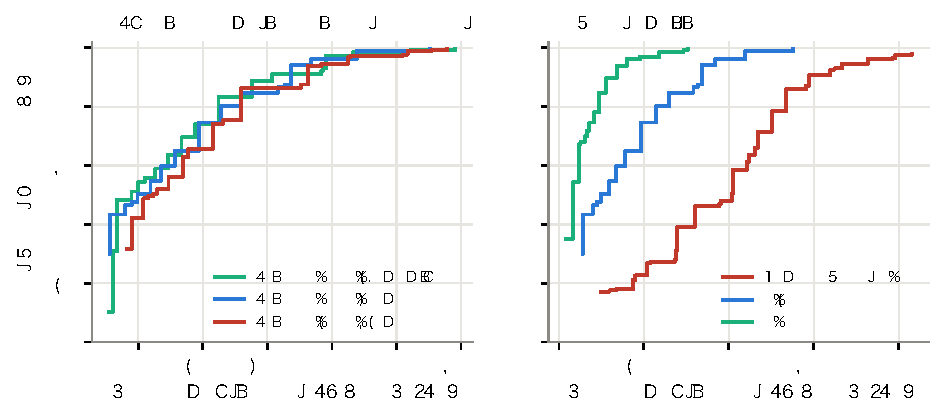
\includegraphics[width=0.98\textwidth]{figs/v6_sensitivity.pdf}
\caption{Best Target Coverage over all initial actions and rules against mean cumulative cost (256 evaluation scenarios). (a) Prior mean of the forecast (planning assumption); the true climates are the same. (b) Damage target (1.0, 1.2, 1.4 × the no-measure damage in the current climate).}
\label{fig:sens}
\end{figure}

\begin{table}[tbp]
\centering\small
\caption{Sensitivity to the planning assumption and the Target (256 evaluation scenarios; costs: mean cumulative cost, PV [100 M JPY]). ``Cheapest path to $\ge$98\%'': initial action with the lowest cost among the rules reaching Coverage $\ge$ 98\%}
\label{tab:sens}
\resizebox{\textwidth}{!}{\begin{tabular}{@{}lrrrrr@{}}
\toprule
Case & No measures & Paddy-field dams only & \multicolumn{2}{c}{Cheapest path to $\ge$98\%} & Levee in the initial action \\
 & max Coverage & max Coverage & Initial action (initial cost) & Cost & max Coverage (cost) \\
\midrule
Base (prior ×1.10, 0.38 m; Target 1.2) & 46\% & 99\% & Paddy-field dams (20) & 438 & 98--100\% (551--705) \\
Mild prior (×1.05, 0.29 m) & 46\% & 99\% & Paddy-field dams, raising, storage (112) & 512 & 98--100\% (522--663) \\
Severe prior (×1.25, 0.62 m) & 46\% & 91\% & Paddy-field dams, storage (56) & 517 & 98--100\% (556--578) \\
Target 1.0 & 4\% & 70\% & Levee down +1 m, paddy-field dams, raising, storage (483) & 831 & 92--98\% (800--888) \\
Target 1.4 & 94\% & 100\% & Paddy-field dams (20) & 236 & 98--100\% (432--518) \\
\bottomrule
\end{tabular}}
\par\footnotesize The initial actions are re-derived for each prior (the planner's nominal world changes); the Target cases use the base initial actions.
\end{table}

\begin{itemize}
  \item \textbf{計画時の想定（予測の事前分布）}: 事前分布の平均を ×1.05・0.29 m（穏やか）または ×1.25・0.62 m（厳しい）に変えても（真の気候は同じ）、
    Coverage と費用の関係はほとんど変わらない（図\ref{fig:sens}(a)）。施策なしの上限は 46\%、Coverage 98\% 以上に要する費用は 438〜517 億円である（表\ref{tab:sens}）。
    ルールは学習で更新される予測を監視するため、事前分布の偏りは意思決定の時点で多くが補正される。
  \item 想定が変えるのは初期行動の候補である（候補は計画者の標準値の世界で選ぶため）。堤防を含む候補は基準 5、穏やか 4、厳しい 3 で、厳しい想定では移転・各戸貯留・ポンプを多く含む候補が増える。
    どの想定でも、「安い初期行動から堤防を加える」経路と「堤防を最初に含む」経路の両方が Coverage 98\% 以上に達する。
  \item \textbf{Target の水準}: Target は結果を大きく変える（図\ref{fig:sens}(b)）。被害額 1.0 倍（現在の被害を増やさない）では、施策なしの Coverage は 4\%、田んぼダムだけから始めると 70\% が上限で、
    Coverage 90\% 以上に達するのは下流堤防 +1 m を最初から含む初期行動（\#1・\#8・\#10・\#11; 92〜98\%、費用 800〜888 億円）だけである。早い段階の備えが必要になる。
  \item 被害額 1.4 倍では、施策なしでも Coverage 94\% で、田んぼダム（\#7）から始めると 98\% を 236 億円で得る。堤防を最初に含む初期行動は 432〜518 億円で、安い初期行動の方が明らかに有利である。
  \item したがって、初期に大きく投資すべきかどうかは、気候の想定よりも Target の水準（どの被害の増加を許容するか）で決まる。
\end{itemize}
